\subsubsection{設計レビューと監査}

\term{設計レビュー}{Design Review} は、設計を包括的に調べる活動である。目的は、設計の完成度、要求の網羅、未解決事項、潜在問題、品質リスクを確認することである。レビューは、設計チーム自身、独立した第三者、顧客、品質保証担当などによって行われる。

\term{設計監査}{Design Audit} は、より狭い観点に焦点を当てる。たとえば、特定の機能監査、標準への適合監査、セキュリティ方針への適合監査などである。

\begin{figure}[htbp]
\centering
\IfFileExists{assets/fig-ch03-11.png}{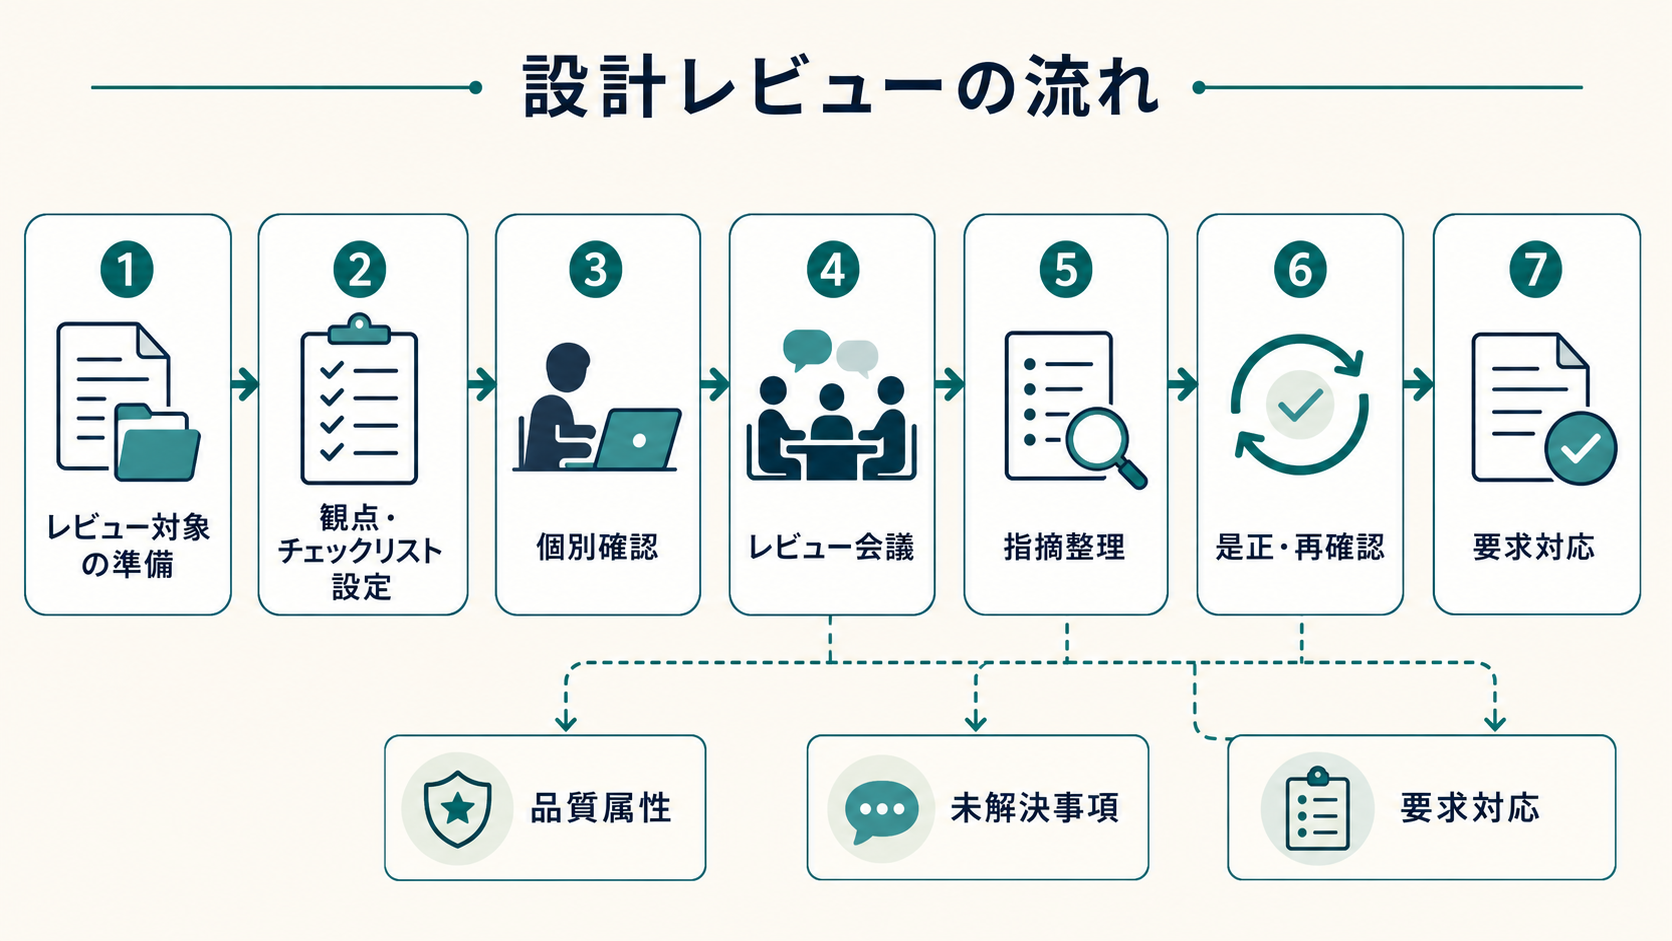
\includegraphics[width=0.96\linewidth]{assets/fig-ch03-11.png}}{\fbox{\parbox[c][48mm][c]{0.9\linewidth}{\centering 画像生成待ち\\設計レビューの流れ}}}
\caption{設計レビューの流れ}
\label{fig:ch03-11}
\end{figure}
